\documentclass{article}
\usepackage[utf8]{inputenc}
\usepackage{float}

\title{Distributed computing assignment 1: SOA}
\author{Zhong-Xi Lu, Angela Mizero, Thomas Van Bogaert}
\date{}

\usepackage{natbib}
\usepackage{graphicx}

\begin{document}

\maketitle

\section{Service Oriented Architecture}

\begin{figure}[H]
    \centering
    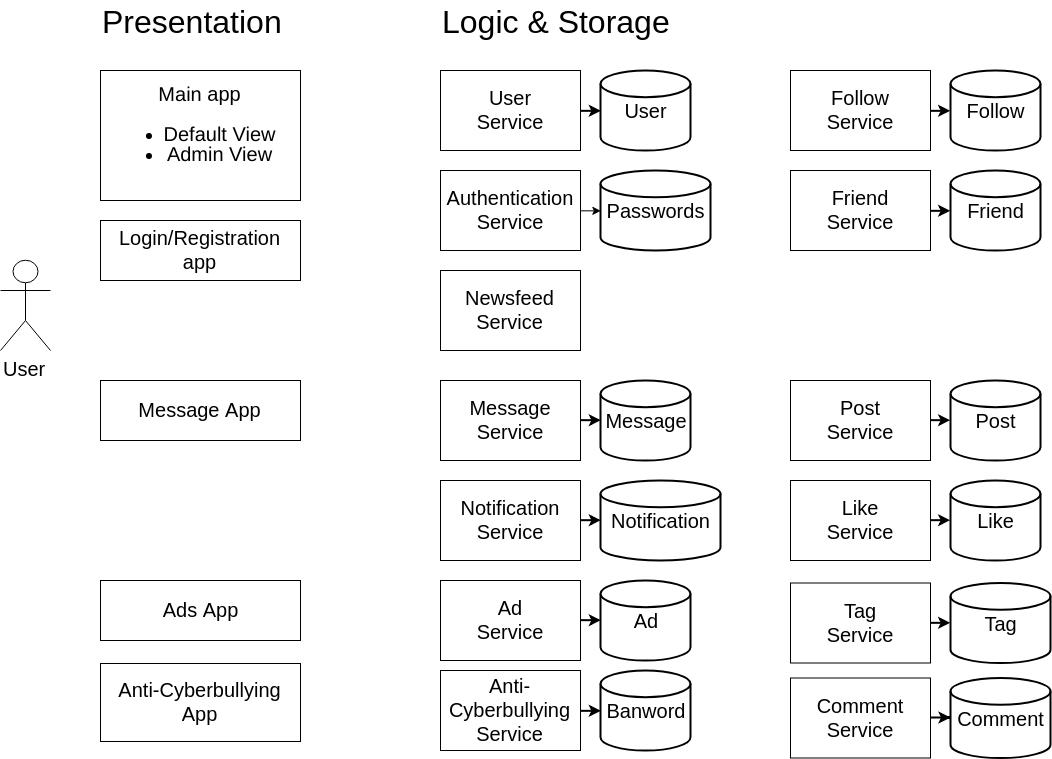
\includegraphics[width=\textwidth]{DC.png}
    \caption{Service oriented architecture}
    \label{soa}
\end{figure}

\section{API Services}

\begin{description}
    \item [Notification service:] 
    \begin{description}
        \item[]
        \item[In:] POST (notification contents, notification recipient(s) (UID))
        \item[Out:] /
        \item[Logic:] Add notification to DB
        \item[]
        
        \item[In:] GET getnotifications/user\_id 
        \item[Out:] Notifications (ID, Timestamp, Content)
        \item[Logic:] Mark notification as requested
        \item[]
        
        \item[In:] PUT removenotification/notification\_id/user\_id
        \item[Out:] /
        \item[Logic: ] Mark notification as read
    \end{description}
\end{description}

\begin{description}
    \item [Post service:] 
    \begin{description}
        \item[]
        \item[In:] POST posts (creator, content, tags)
        \item[Out:] /
        \item[Logic:] Create a new post
        \item[]

        \item[In:] GET posts/user/user\_id
        \item[Out:] Posts (creator, timestamp, content, tags)
        \item[Logic:] Get all the posts from a user
        \item[]

        \item[In:] GET posts/post\_id
        \item[Out:] Post (creator, timestamp, content, tags)
        \item[Logic:] Get a specific post
        \item[]
        
        \item[In:] POST posts/post\_id/like (user\_id)
        \item[Out:] /
        \item[Logic: ] User likes a post
    \end{description}
\end{description}

\begin{description}
    \item [Tag service:] 
    \begin{description}
        \item[]
        \item[In:] POST tags (post\_id, user\_id(s))
        \item[Out:] /
        \item[Logic:] Create a user tag on a specific post
        \item[]
        
        \item[In:] GET tags/tag\_id
        \item[Out:] tag (tag\_id, post\_id, user\_id)
        \item[Logic:] Get a specific tag
        \item[]

        \item[In:] GET tags/posts/post\_id
        \item[Out:] Tags (tag\_id, post\_id, user\_id)
        \item[Logic:] Get all the tags on a post
        \item[]
    \end{description}
\end{description}

\begin{description}
    \item [Comment service:] 
    \begin{description}
        \item[]
        \item[In:] POST comments (post\_id, creator, content)
        \item[Out:] /
        \item[Logic:] Create a comment on a specific post
        \item[]
        
        \item[In:] GET comments/comment\_id
        \item[Out:] Comment (comment\_id, creator, timestamp, content)
        \item[Logic:] Get a specific comment
        \item[]

        \item[In:] GET comments/posts/post\_id
        \item[Out:] Comments (comment\_id, creator, timestamp, content)
        \item[Logic:] Get all the comments on a post
        \item[]
    \end{description}
\end{description}

\end{document}
